Understanding when clinical events occur is fundamental to modeling patient trajectories, enabling tasks such as process mining, outcome forecasting, and causal inference in medicine \citep{jensen2012mining, noren2010temporal}.
However, most clinical narratives lack explicit temporal structure. While electronic health record (EHR) datasets like MIMIC-III and MIMIC-IV include timestamped structured data and clinical notes \citep{johnson2016mimic, johnson2023mimic}, they capture only a subset of events (e.g., vital signs, lab results) and still require sophisticated natural language processing to extract temporal information from unstructured text \citep{viani2021temporal, cheng2023typed}.


In contrast, published case reports often provide rich narrative descriptions of patient timelines, but the timing of events is typically expressed in relative terms within the free text (e.g., “on day 3 of hospitalization”).
Efforts in temporal reasoning on clinical text have been hampered by the scarcity of large-scale annotated corpora.
Earlier initiatives, such as the 2012 i2b2 challenge and Clinical TempEval, focused on temporal relation extraction from clinical notes \citep{sun2013evaluating, bethard2016semeval, galvan2018investigating} but were constrained by small datasets (e.g., 310 documents) from single institutions, limiting model performance and generalizability.
Systems that rely on metadata timestamps (e.g., admission or discharge dates) fail to capture the fine-grained sequence of clinical events described in text, which is essential for nuanced understanding and prediction.
There remains a pressing need for large-scale, temporally annotated corpora to support the development and evaluation of models for clinical temporal reasoning.

Building on our pilot pipeline on 20 case reports \citep{wang2025large}, we introduce the PubMed Open Access Textual Time Series (PMOA–TTS) corpus—a large-scale dataset of 124,699 openly available clinical case reports, each annotated with a structured timeline of events.
Leveraging large language models (LLMs)—specifically \texttt{Llama 3.3} \citep{grattafiori2024llama} and \texttt{DeepSeek-R1} \citep{guo2025deepseek}—we transform each case report into a sequence of \mbox{(clinical event, time)} tuples that capture key clinical events and their relative timing within the patient narrative (Figure \ref{fig:annotation_ex}).
To our knowledge, PMOA–TTS constitutes the largest publicly available collection of clinical narratives with explicit temporal event structure.
We demonstrate that these temporal annotations enable novel forms of analysis and significantly enhance downstream modeling of patient outcomes.


Building PMOA--TTS requires addressing three challenges at scale: reliably identifying single-patient case reports, extracting timeline events with high fidelity from ambiguous free-text time expressions, and rigorously evaluating the resulting annotations. We meet these needs with an LLM-based pipeline that selects relevant narratives beyond naive metadata filters, resolves relative time language into fine-grained event--time tuples, and enriches each case with structured demographics and diagnoses. To illustrate practical value, we also formulate a downstream survival analysis task that operates directly on the extracted textual time series.

% \begin{figure}[!htbp] % 'r' for right, 'l' for left
%     \centering
%     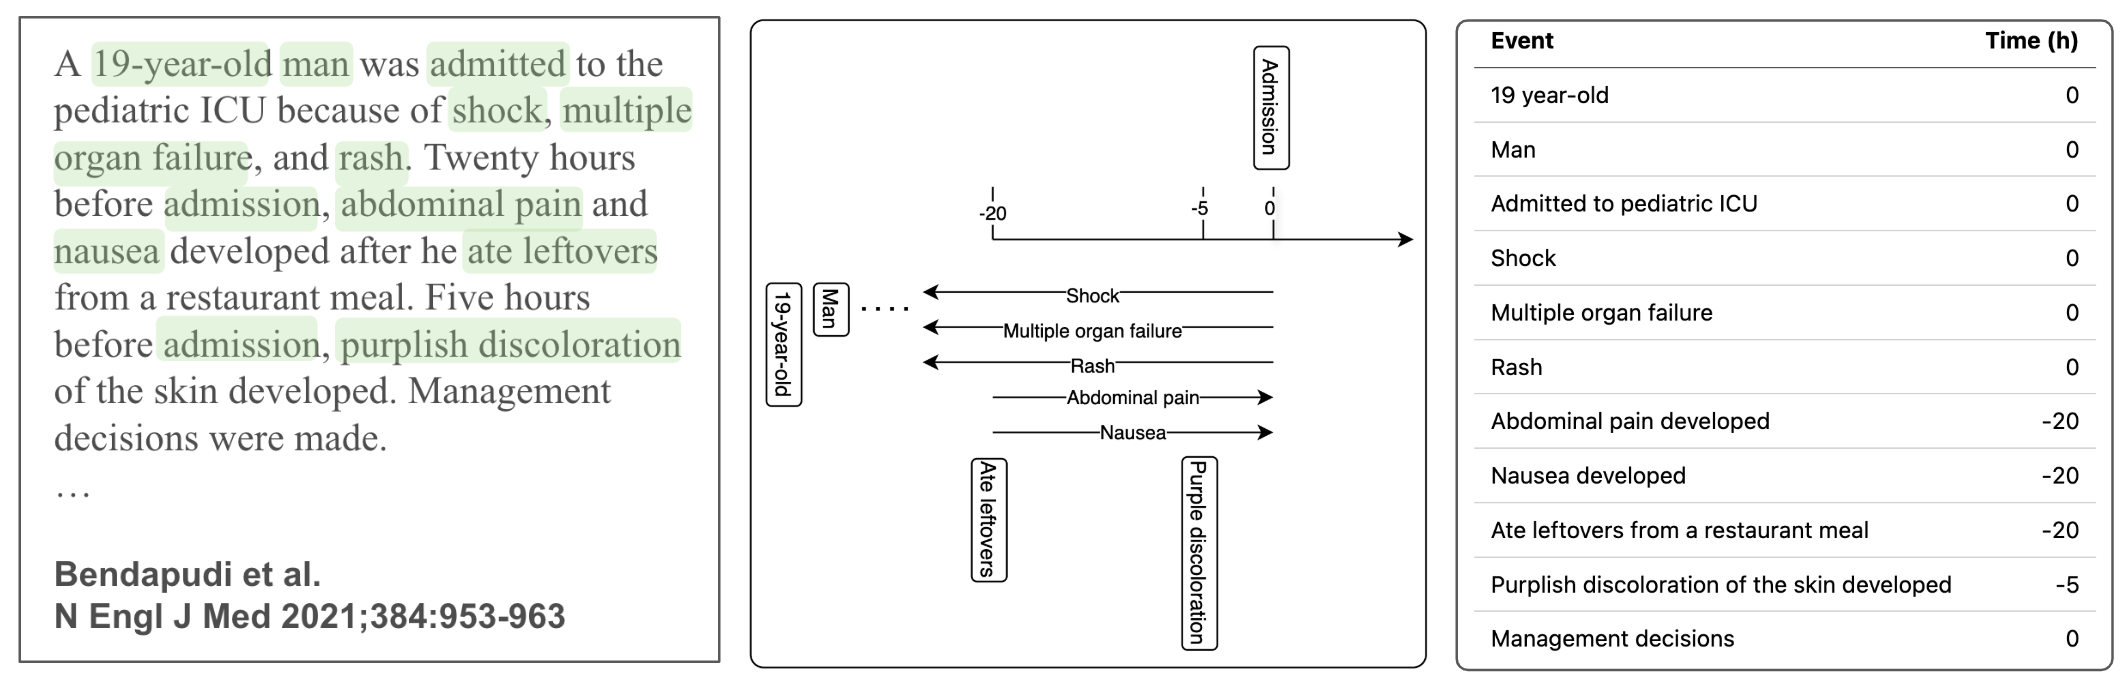
\includegraphics[width=\linewidth]{Plots_tables/annotation_ex.png} % Adjust width
%     \caption{Example case report (left) with temporal representations as timelines (middle) and text-ordered, event-time tuples (right).\textcolor{red}{Figure already in forecasting paper, change if needed.}}
%     \label{fig:annotation_ex}
%     \vspace{-2.5mm}
% \end{figure}

\begin{figure*}[t]
  \centering

  % ---- Left panel: narrative (boxed) ----
  \begin{subfigure}[t]{0.49\textwidth}\vspace{0pt}
  %\begin{subfigure}[t]{0.48\linewidth}\vspace{0pt}
    \begin{tcolorbox}
    [
    colback=white,
    colframe=black!30,
    arc=2mm,
    boxrule=0.6pt,
    left=2mm,right=2mm,top=2mm,bottom=2mm
    ]
      \small\raggedright
      A \hl{52-year-old} \hl{woman} was \hl{admitted to the medical ICU} with \hl{chest pain} and \hl{shortness of breath}. She developed \hl{intermittent fever and fatigue} a couple of weeks prior to admission. Eight hours after hospital and ICU admission, \hl{broad-spectrum antibiotics} were \hl{started for suspected infection}. On hospital admission day 2, she developed \hl{pleuritic pain} and \hl{escalating oxygen requirements}. \hl{CT angiography} was performed two days after admission.
      
    \end{tcolorbox}
    \caption{Case narrative with highlighted clinical events}
    \label{fig:narrative_box}
  \end{subfigure}\hfill%
  % ---- Right panel: event–time table (boxed) ----
  \begin{subfigure}[t]{0.49\textwidth}\vspace{0pt}
  %\begin{subfigure}[t]{0.48\linewidth}\vspace{0pt}
    \begin{tcolorbox}
    [
    colback=white,
    colframe=black!30,
    arc=2mm,
    boxrule=0.6pt,
    left=2mm,right=2mm,top=2mm,bottom=2mm
    ]
      \small\centering
      \setlength{\tabcolsep}{5pt}
      \begin{tabular}{@{} l r @{}}
        \toprule
        \textbf{Event} & \textbf{Time (h)} \\
        \midrule
        52-year-old & 0 \\
        woman & 0 \\
        admitted to the medical ICU & 0 \\
        chest pain & 0 \\
        shortness of breath & 0 \\
        developed intermittent fever & -336 \\
        developed fatigue & -336 \\
        broad-spectrum antibiotics started \\ for suspected infection & 8 \\
        pleuritic pain developed & 24 \\
        escalating oxygen requirements & 24 \\
        CT angiography & 48 \\
        %Management decisions & 48 \\
        \bottomrule
      \end{tabular}
    \end{tcolorbox}
    \caption{Text-ordered event–time tuples.}
    \label{fig:table_box}
  \end{subfigure}

  \caption{Example case report (left) with text-ordered event-time tuples (right).
  }
  \label{fig:annotation_ex}
  \vspace{-5mm}
\end{figure*}






In summary, we (i) introduce the PMOA Textual Time Series (PMOA--TTS) corpus of 124{,}699 single-patient case reports from PubMed Open Access, each annotated with structured clinical timelines extracted using large language models; (ii) develop a scalable pipeline for automatic case identification and prompt-driven extraction of timelines, demographics, and diagnoses, together with a manual evaluation framework; (iii) define and apply complementary validation measures for timeline accuracy, including temporal order concordance (c-index) and the Area Under the Log-Time CDF (AULTC); (iv) characterize corpus properties (demographics, frequent diagnoses, and co-occurrence structure) to document clinical and demographic breadth; and (v) illustrate one reuse pathway by framing survival prediction directly over textual time series.


% PMOA--TTS fills a critical gap by providing a large-scale, openly available resource for temporal reasoning in clinical narratives. It is intended to support (1) improved timeline extraction and temporal reasoning from free text; (2) survival analysis and risk stratification using textual time series representations; and (3) event forecasting and temporal question answering across diverse conditions. The case-mix breadth and extracted attributes enable cohort assembly without new annotation, while the corpus scale supports robust evaluation of temporal methods. Example downstream formulations (survival and forecasting) show how textual time series can be operationalized, while the dataset itself remains task-agnostic. Together, these elements position PMOA--TTS as a reusable, openly available foundation for temporal NLP in biomedicine, complementing EHR-based resources and enabling work that requires explicit event sequences from narrative clinical text.

The PMOA–TTS corpus offers several potential positive contributions to the biomedical NLP and clinical AI communities. By releasing the largest openly available dataset of temporally structured clinical narratives, this work democratizes access to timeline-based clinical text—an area typically limited to proprietary EHR datasets. The corpus spans a wide range of diagnoses and demographics, supporting research on temporal patterns in diverse and sometimes underrepresented conditions. Additionally, by making the extraction pipeline, prompting strategies, and evaluation framework publicly available, the project promotes transparency and reproducibility in LLM-based clinical information extraction. These contributions collectively advance the development of models for timeline reconstruction, temporal reasoning, and longitudinal prediction, while lowering the barrier
to entry for researchers working in resource-limited settings.

% \begin{itemize}
%     \item \textcolor{red}{Contributions as bullet points or paragraph? Bullet points is more CS style}
%     \item \textcolor{red}{Do we need more related works in background? Only included related work about "clinical narrative datasets" and "temporal NLP" since these are most relevant to the dataset.}
%     \item \textcolor{red}{NeurIPS DB had a separate Appendix section "Broader impact". Tried to describe impact in background only. Do we need separate section in Appendix?}
% \end{itemize}

% The rest of the paper is organized as follows: \textbf{Methods} describes the procedures used to create the dataset. \textbf{Data Records} documents the resource itself—where it is hosted, how the files are organized, and the formats used. \textbf{Technical Validation} reports the analyses performed to verify and support the dataset’s technical quality. \textbf{Usage Notes} provides practical guidance to help others reuse the data. \textbf{Dataset Availability} and \textbf{Code Availability} states where the code for generating the data is hosted and the conditions under which it can be accessed.

%%%%%%%%%%%%%%%%%%%%%%%%%%%%%%%%%%%%%%%%%
%%%%%%%%%%%%%%%%%%%%%%%%%%%%%%%%%%%%%%%%

